\chapter{Application to bootleg detection}
\label{Chap:Bootleg}
In the past few years, the Web has been characterized by an exponentially increasing trend of democratization, since people are now invited to participate in the information sharing process. This also includes the possibility of distributing multimedia content (such as audio, images, and video files) through one of the many media sharing platforms (e.g., SoundCloud, YouTube, etc.). The media sharing process has clearly been eased by the diffusion of inexpensive portable devices (such as camcorders and smartphones) that enable anyone to produce their own audio-visual content. However, besides the positive advantages given by the opportunity of sharing user-generated content, a certain form of regulation is often needed to avoid unpleasant situations. Indeed, it is not rare to hit on tampered media or illegally distributed material while surfing the Web.

Distribution of forged multimedia content is nowadays a serious threat. As an example, newscasts may broadcast (either intentionally or unintentionally) fake videos or images, with the severe consequence of conveying false (and maybe biased) information. Nonetheless, the illegal distribution of copyrighted material is another major issue. Indeed, movie and audio piracy damages both artists and entertainment industries.

To solve such problems related to media authentication and verification, the multimedia forensics community has developed a series of algorithms to work with audio \cite{Gupta2012}, images \cite{Piva2013}, and videos \cite{Milani2012}. These algorithms can be roughly divided into two categories: \textit{active} methods that rely on the injection of some sort of signatures into an object before its distribution \cite{Cox2008,Chena2012,Wang2014}; and \textit{blind} methods that aim at passively verifying the integrity of an object, relying only on traces left by processing operations \cite{Mahdian2010,Dittmar2012}. 

One of the main problems with audio content is the unauthorized recording of live performances, called \textit{bootlegs} \cite{Bestagini2013b}. In this Chapter, we address the problem of designing a tool to automatically detect audio bootlegs with a blind approach. This tool is useful to detect the presence of illegal or unauthorized material on media sharing platforms, therefore to provide an automatic description of audio pieces in music collections. The bootleg detection problem has been extensively studied as far as it concerns the re-distribution of video sequences acquired in cinemas and theaters. In this scenario, many active \cite{Haitsma2001,Doerr2003,Robert2013} and passive \cite{Visentini-Scarzanella2012,Bestagini2013a} methods have been proposed over the years. Some investigations have also been carried out to address audio-related forensics problems. In \cite{Peters2012} the authors exploit audio cues to estimate the used recording room. More recently, in \cite{Milani2014}, a method to disambiguate between indoor and outdoor audio recordings has been proposed. Other closely related works aim at estimating the specific model of the used audio acquisition device. To this purpose, in \cite{Garcia-Romero2010} an algorithm for device identification based on speech recordings is proposed. In \cite{Cuccovillo2013}, the authors show how to identify the portable device used for a given recording. However, only the work in \cite{Bestagini2013b} strictly copes with audio bootlegs in the literature.

In this scenario, we design a linking function that detects semantic characteristics of the recordings from their audio signals. The semantic domain is formalized following a disjoint categorical approach, to detect whether a certain track is a bootleg. Since the bootlegs are unauthorized recordings of live performances, it is reasonable to define the semantic domain with three non-overlapping labels for officially released studio album, live album and unofficial bootleg recordings. The signal domain is instead uncertain, since it is hard to identify which acoustic properties are affected by the recording of bootlegs. Due to such uncertainty of the signal domain, it is not possible to define the linking function as a rule-based technique. We address the bootleg detection problem by using unsupervised learned features to represent the signal domain and machine learning techniques to classify the music tracks into one of the three aforementioned categories.

The proposed approach is similar to the one proposed in \cite{Bestagini2013b}. The main differences with respect to \cite{Bestagini2013b} are:
\begin{enumerate}
\item \cite{Bestagini2013b} proposes two classes to define whether a certain audio track is a bootleg recording, while we use three classes in order to provide a richer description of the semantic domain;
\item we use an unsupervised feature learning approach, while \cite{Bestagini2013b} employs hand-crafted features from a large set of acoustic and structural cues from different domains (energy, timbre, harmony, etc.)\cite{Kim2005}.
\end{enumerate}
In \cite{Bestagini2013b} the authors model the linking function as a Support Vector Machine (classifier); in this work, we follow the same approach for comparison purposes.

We validate our proposed approach for bootleg detection against a set of nearly 500 songs of different genres and artists. Results show that the novel architecture greatly outperforms the model proposed by \cite{Bestagini2013b} and it achieves almost perfect performance on the bootleg detection problem. This research was presented at the IEEE International Workshop on Information Forensics and Security \cite{buccoli2014}.  



 \begin{figure}[tbp]
    \begin{center}
      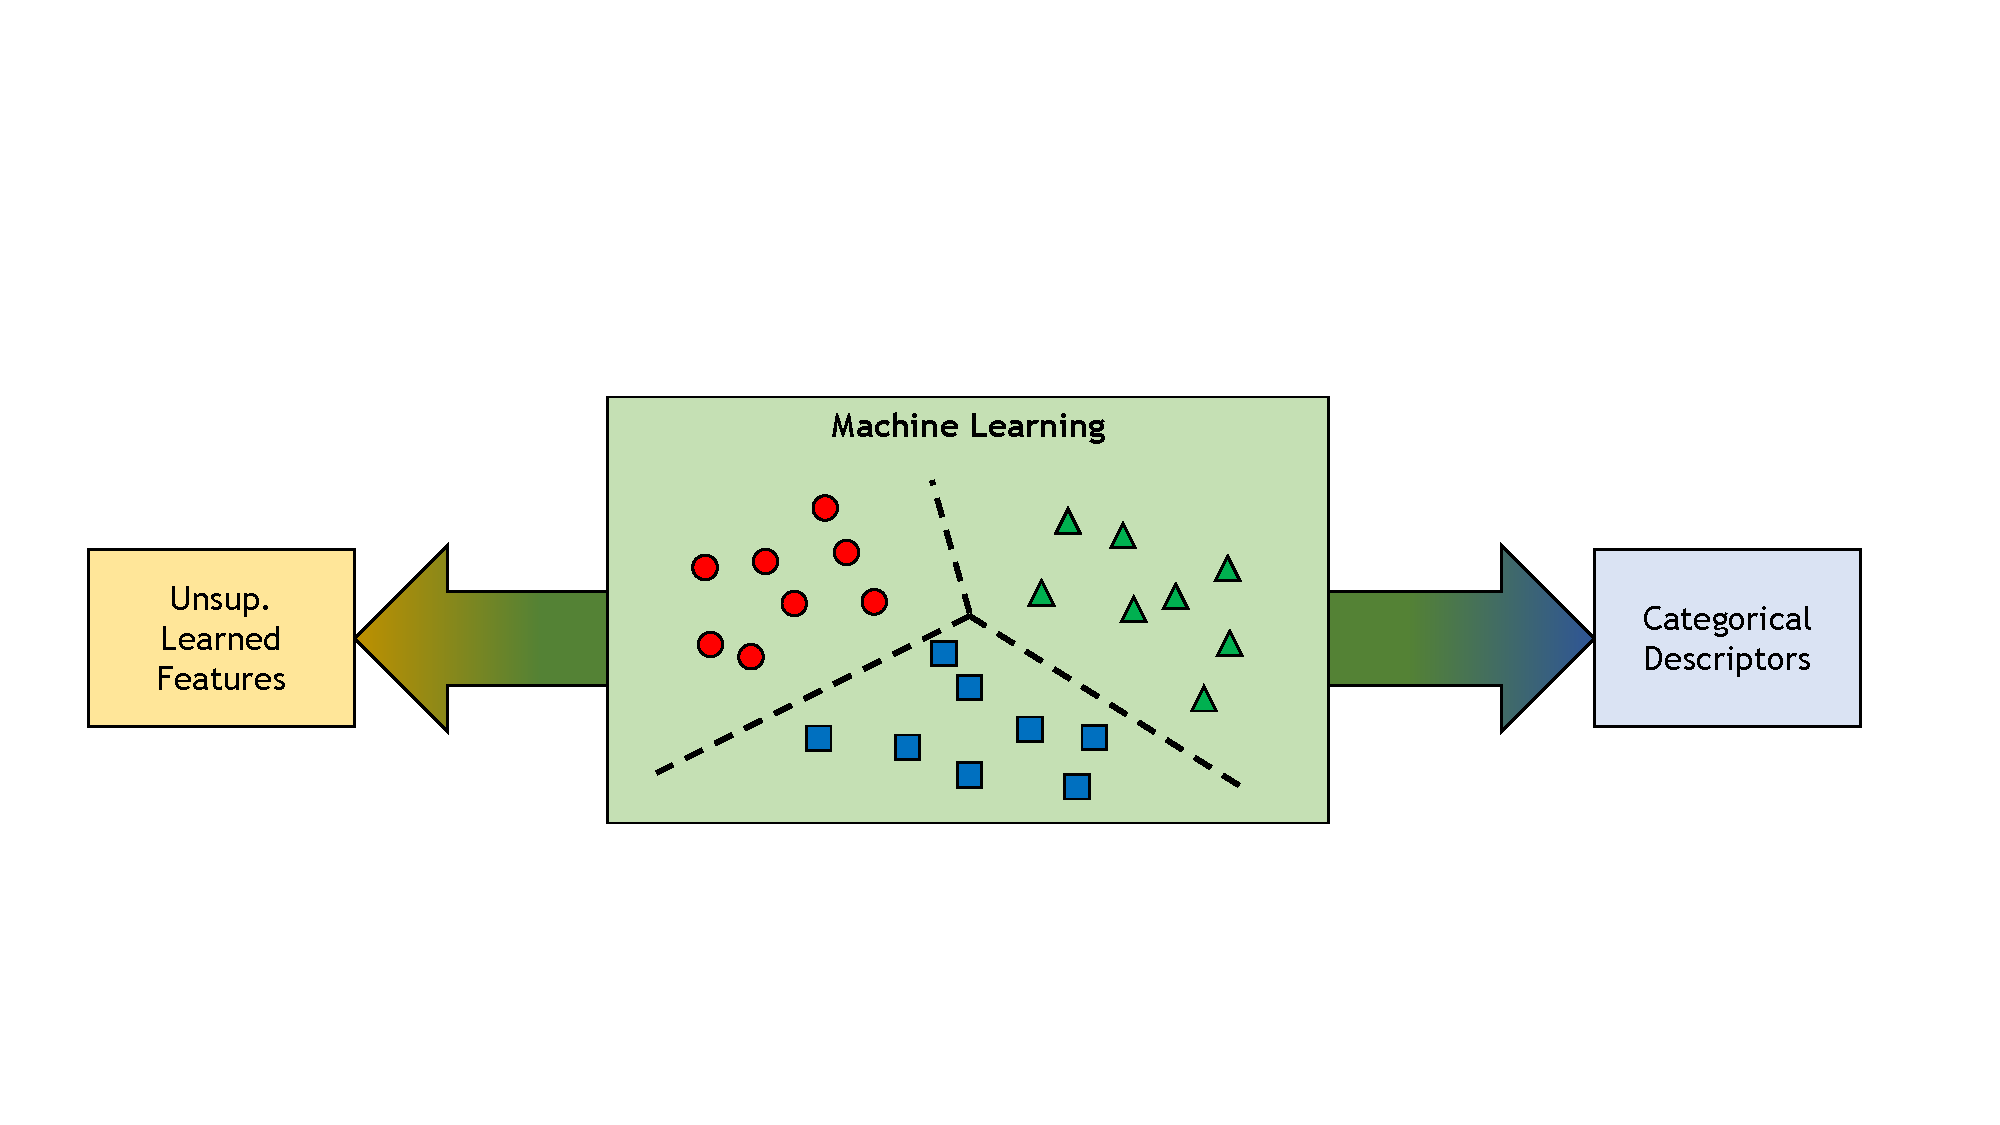
\includegraphics[trim=1cm 5cm 2.3cm 6.5cm,clip=true,width=\textwidth]{img/Bootleg/schema}
	%\psfig{file=im/ML/logopm.jpg,width=3.5cm}
    \end{center}
  \caption{The scheme of the proposed bootleg-detection application scenario}
  \label{fig:Bootleg:scheme}
  \end{figure}

In Figure \ref{fig:Bootleg:scheme}, we show the block diagram of the proposed approach for the supervised classification of the musical content, based on the formalization of the music signal with unsupervised learned features. In the following Sections, we provide an overview on the characterization of audio bootlegs. We then discuss our experimental setup and the numerical results we obtain, with a direct comparison with the results achieved by \cite{Bestagini2013b}. Finally, we draw some conclusions on the work.

\begin{figure}[t]
\centering
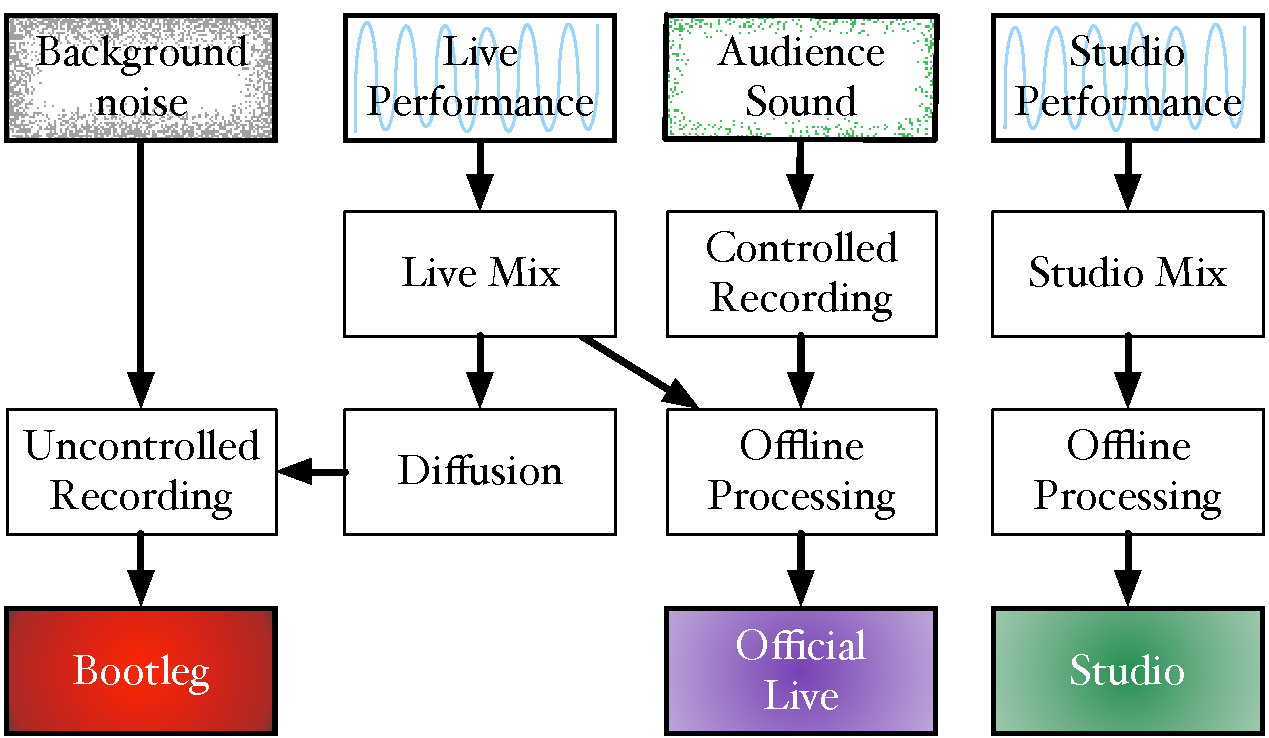
\includegraphics[width=1\columnwidth]{img/Bootleg/paolo_figu}
\caption{Diagram representing the main contributions and processing in Bootleg, Live and Studio recordings generation.}
\label{fig:Bootleg:schema}
\end{figure}
\section{Characterization of the semantic domain of audio bootlegs}\label{sec:Bootleg:overview}
In this study we formalize the semantic domain by means of three non-overlapping classes, namely \textit{bootleg} ($\B$), \textit{studio} ($\S$), and \textit{official live} ($\O$). Songs belonging to different classes undergo different processing steps during acquisition, editing and mastering. Each operation leaves peculiar traces on the recordings that are an asset for our detector. In order to better understand the nature of footprints left on different audio tracks, let us consider each class separately.  

\textit{Official live} relates to professional recordings of live concerts. The recording is performed by setting up proper audio consoles that allow to acquire separate tracks from different microphones or other audio sources. Tracks are then edited and mixed off line. 
Thanks to post-processing operations, the sound is well balanced and well defined, though it is characterized by the presence of environmental sounds like crowd voices, claps, screams, etc. Nevertheless, thanks to the multi-track recording technique, the environmental effects are well controlled. 

\textit{Bootleg} recordings are performed through non-professional or semi-professional engines. The sound diffused by the speakers is acquired with some built-in microphones from the audience. \textit{Bootlegs}, with respect to \textit{official live} recordings, present a sound highly altered by the acquisition position in the audience. The mutual position between microphones and loudspeakers may induce unwanted phase effects and the sound may be affected by the acoustic response of the environment. Moreover, they are recorded in very loud, uncontrolled and possibly noisy environments, with low or mid-level equipment that are not designed for high-quality music recording. For these reasons, \textit{bootlegs} tend to exhibit clipping effects, rumblings, and a worse balanced sound. Environmental sounds are also present, but, clearly, they cannot be controlled and this leads to a degradation of the overall quality of the recordings. 

\textit{Studio} songs are obtained by professionally recording music pieces in a controlled and noiseless environment. Tracks are edited and mixed, optionally applying audio enhancement effects. Such tracks play very clear, exhibit a high signal-to-noise ratio and do not present noise from the audience.


\section{Characterization of the signal domain of audio bootlegs}\label{sec:Bootleg:signal}
In order to properly characterize audio content, and hence to be discriminative with respect to the three classes, content-based classical approaches consider the extraction of hand-crafted and model-based features from the audio signal \cite{Kim2005}.
%highly-discriminant sets of audio cues (audio features) from the audio signal \cite{Kim2005}. 
These features are chosen in order to capture specific aspects of the sound to analyze, the ones used  by the human ear to discriminate and isolate sounds \cite{Kim2005,Zanoni2012}.
%. In this approach, the rationale is to select the most relevant set of features. The set of features is generally manually chosen. For this reason we will refer to them as \textit{hand-crafted} features. The intent is to select the set of features used by the human ear to discriminate and isolate sounds \cite{Kim2005,Zanoni2012}. 
In the work by \cite{Bestagini2013b}, the authors analyze a set of classic hand-crafted features, which is listed in Table \ref{tab:Bootleg:LLFs} (see Section \ref{sec:LLFs:hand-crafted} for a formalization of most of them). The basic idea is to select which characteristics are involved in the generation of the bootleg recordings and extract the features that capture such characteristics.  However, it is not clear which features are affected by the bootleg recordings. For this reason,  we use an approach based on unsupervised feature learning, by means of a Deep Belief Network (DBN) similar to the one described in Chapter \ref{Chap:MSA}.

The DBN provides a feature representation for the different layers of which it is composed, with each layer extracting a different level of abstraction from the audio signal. In this work, we are interested in comparing the performance obtained with hand-crafted and learned features. The hand-crafted feature have one main advantage over the learned ones: they can be interpreted to better understand which underlying aspects are more relevant for the addressed problem. Nevertheless, we can similarly analyze the performance obtained with the features extracted from the different layers of the DBN. In this work, we perform such analysis, in order to better understand which underlying level of abstractness is required to address the task of bootleg detection

We first collect a set $\mathcal{S}$ composed of 480 well-known songs sampled at the standard audio sampling frequency of 44100 Hz and selected to cover a big set of music genres (e.g., rock, classic, jazz, etc.). With regard to bootlegs, we collect them from different sources, including YouTube and sharing fan sites, and we aim at covering a wide variety of recording conditions (e.g., noisy concert halls, small clubs, etc.). 

It is common, in the production stage, to mix the stereo channels with different approaches for studio or live tracks. Using such information on the stereo channels might be useful to classify the songs, but it might also lead to overfit the linking function to these approaches. For this reason, we choose to convert the tracks in mono and in order to focus on the audio content and to generalize the proposed solution by avoiding possible overfitting.
The songs are equally distributed into three classes: i) \textit{bootleg} ($\B$); ii) \textit{official live} ($\O$); iii) \textit{studio} ($\S$). Each class is composed of 160 songs belonging to different artists and four different genres (i.e., blues, metal, pop, and rock). In order to speed up our analysis, each song is trimmed to 30 seconds, taken from the middle of the track. We split the entire dataset into three disjoint sets: i) $\Sdbn$ to train the DBN; ii) $\Ssvm$ to train the SVM classifier; iii) $\Stest$ to test the performances of the detector. Each set contains songs belonging to every class.

\begin{table}[t!]
\caption{List of the hand-crafted features used in \cite{Bestagini2013b}.}
\label{tab:Bootleg:LLFs}
\centering
%\scriptsize
\large
\bgroup
\def\arraystretch{1.5}
\begin{tabular}{||p{0.15\textwidth}|p{0.75\textwidth}||}
\hline
\hline
\textbf{Property} & \textbf{Features}\\ 
\hline
\hline
\textit{Frequency response} & Spectral Centroid, Spectral Spread, Spectral Kurtosis, Spectral Skewness, Spectral Flux, Spectral Rolloff, MFCC \\
\hline
\textit{Inharmonic Distortion}    & Spectral Irregularity, Spectral Entropy,
Flatness, Zero Crossing Rate \\
\hline
\textit{Harmonic Distortion} & Inharmonicity, Chromagram \\
\hline
\textit{Loudness Saturation} & Spectral Irregularity, Spectral Entropy, Spectral Flatness, Zero Crossing Rate, Energy Root Mean Square \\
\hline
\textit{Background Noise} & Spectral Irregularity, Spectral Entropy,
Spectral Flatness, Zero Crossing Rate \\
\hline
\hline
\end{tabular}
\egroup
\end{table}


\section{Experimental setup and numerical results}
\subsection{Experimental setup}
In order to compute the unsupervised learned features, we use the approach presented in Section \ref{sec:MSA:domains} over the $90$ songs in $\Sdbn$, i.e., with $30$ songs per class. We considered Hamming-windowed frames of 1024 samples, with a 50\% of overlap, for a total of more than 2500 frames per song. We sequentially train a three-layer DBN with 50 neurons per layer, using a pre-training learning rate of $10^{-6}$, and $100$ epochs for each layer. We use more epochs with respect to the case in Chapter \ref{Chap:MSA} since we have less data for the training of the DBN. 

After the training step, we compute feature vectors for every frame of every song in $\Ssvm$ and $\Stest$ : i) $\mathbf{h}^{(1)}_{i,f} \in \mathbb{R}^{50 \times 1}$ from layer 1; ii) $\mathbf{h}^{(2)}_{i,f} \in \mathbb{R}^{50 \times 1}$ from layer 2; iii) $\mathbf{h}^{(3)}_{i,f} \in \mathbb{R}^{50 \times 1}$ from layer 3; iv) $\mathbf{h}^{(all)}_{i,f} = [\mathbf{h}^{(1)}_{i,f}; \mathbf{h}^{(2)}_{i,f}; \mathbf{h}^{(3)}_{i,f}] \in \mathbb{R}^{150 \times 1}$ stacking all the layers' output, where $i$ is the index of a generic song and $f$ is the index for a generic frame. For comparison purpose, we also consider $\mathbf{h}_{i,f}^\text{(hc)} \in \mathbb{R}^{71 \times 1}$ as the vector composed of only hand-crafted features, proposed in the best scenario of \cite{Bestagini2013b}.

Since we extract a feature vector $\mathbf{h}^{(k)}_{i,f}$ for every frame $f$ of each song $i$, we need a strategy to merge them in order to obtain a single feature vector for each song.
As discussed in Section \ref{sec:LLFs:hand-crafted}, several pooling systems for feature vectors have been proposed in order to consider the time-variance nature of music, such as considering the mean, the variance, the maximum, the minimum, and other statistical moments \cite{hamel2011}. We consider the average value of the learned features during the whole song (or excerpt), following the same approach than \cite{Bestagini2013b} with the hand-crafted features. Hence, we average the $\mathbf{h}^{(k)}_{i,f}$ vectors as:
\begin{equation}
\mathbf{h}^{(k)}_i=\frac{1}{F_i} \sum_{f=1}^{F_i} \mathbf{h}^{(k)}_{i,f},
\label{eq:feature}
\end{equation}
where $F_i$ is the number of frames for the $i$-th song.

\begin{figure}[t]
\centering    
\subfloat[Learned Features]{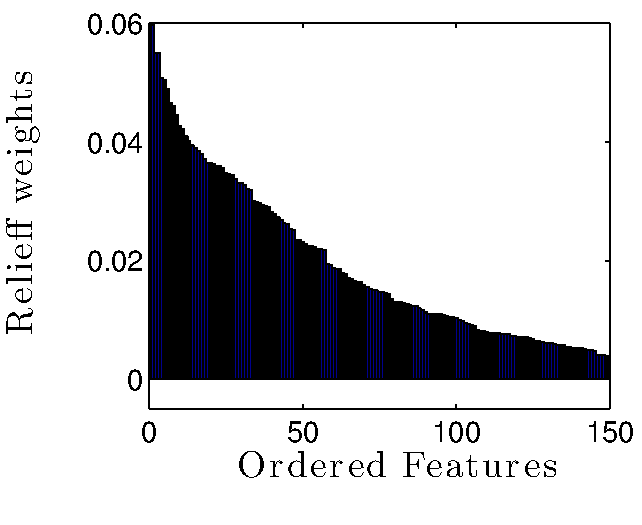
\includegraphics[width=.47\textwidth]{img/Bootleg/dbn_relieff_3}\label{fig:Bootleg:dbn_relieff}} \hfil
\subfloat[Hand-Crafted Features]{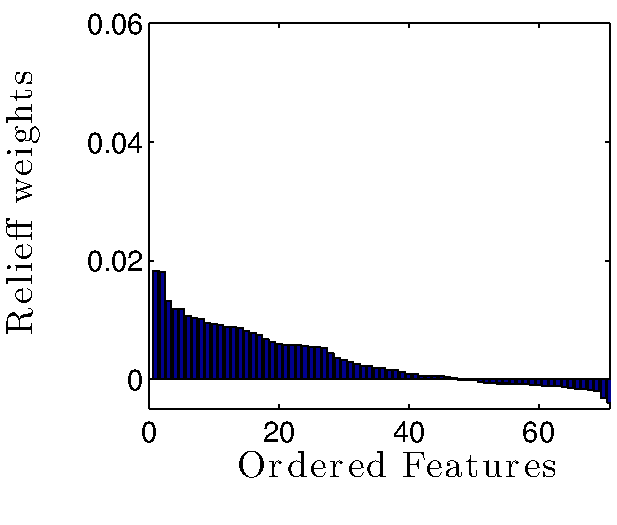
\includegraphics[width=.45\textwidth]{img/Bootleg/classic_relieff_3}\label{fig:Bootleg:classic_relieff}}
\caption{Visualization of Relieff weights for learned (a) and hand-crafted (b) features. Notice how learned features' weights are strictly positive and assume higher values than hand-crafted features.}
\label{fig:Bootleg:relieff}
\end{figure}

To better highlight the discriminable power of $\mathbf{h}^\text{(all)}$ over  $\mathbf{h}^\text{(hc)}$, we also apply the Relieff \cite{Sikonja2003} feature selection algorithm. This algorithm assigns to each feature a weight proportional to the discriminable power of that feature. Figure \ref{fig:Bootleg:relieff} shows the Relieff weights. We notice that features learned from deep architecture are assigned with all strictly positive weights (i.e., are all discriminant), whereas the weights for hand-crafted features have lower values, and about one third of them are negative (i.e., not discriminant for classification). This clearly shows the greater effectiveness of the learned features with respect to the hand-crafted ones in the representation of the signal domain for the bootleg detection problem.

We adopt SVM classifiers considered a classical approach in the literature, also used in \cite{Bestagini2013b}. The details on the SVM classifier are provided in Section \ref{sec:ML:classifiers}. In Section \ref{sec:ML:classifiers} we discussed how the multi-label classification is implemented as a set of $P$ classifier using the one-versus-all approach. This approach, however, can lead to over-fitting issues, due to the uneven distribution of the samples, where the amount samples of the class to be predicted is often
far lower than the amount of the rest of the samples. For this reason,
the one-versus-one strategy, which implements a classifier for each combination of two classes, is sometimes preferred. This strategy is usually rather expensive, since it involves to design $P(P-1)/2$ classifiers. In our scenario with $P=3$ classes, using the one-versus-one strategy is equivalent to use the one-versus-all strategy, while reducing the risk of overfitting.

We train a SVM for every pair of classes, i.e., $\B$ vs $\O$,  $\B$ vs $\S$, and $\O$ vs $\S$. For the sake of simplicity, let us focus on a single SVM, i.e., $\B$ vs $\O$. This SVM takes as input the pairs $(\mathbf{h}_i, y_i), \; s_i \in \Ssvm$, where $y_i \in \{\B, \O\}$. During training, the SVM seeks the manifold in the $M$-dimensional feature space that maximizes the margin between the two classes. This manifold is the decision boundary, which splits the $M$-dimensional space in two regions: songs are detected as belonging to class $\B$ or $\O$ depending on the region within which the feature vector $\mathbf{h}_i$ lies. The distance between $\mathbf{h}_i$ and the manifold boundary is the likelihood value of the $i$-th song to belong to the associated class. We repeat the training step for each SVM. In order to exploit nonlinearity in the design of the manifold, we use a RBF kernel for the training of the SVM classifiers (see Section \ref{sec:ML:kernels}).

After the training we  use the three SVM models on test songs to detect their class, i.e., $\B$, $\O$, or $\S$. More specifically, each SVM returns the likelihood of the song to belong to each class as the distance from the correspondent feature representation to the decision manifold. The class with the highest likelihood is associated with the song. 

\begin{figure}[tbp]
\centering
\subfloat[Learned Features]{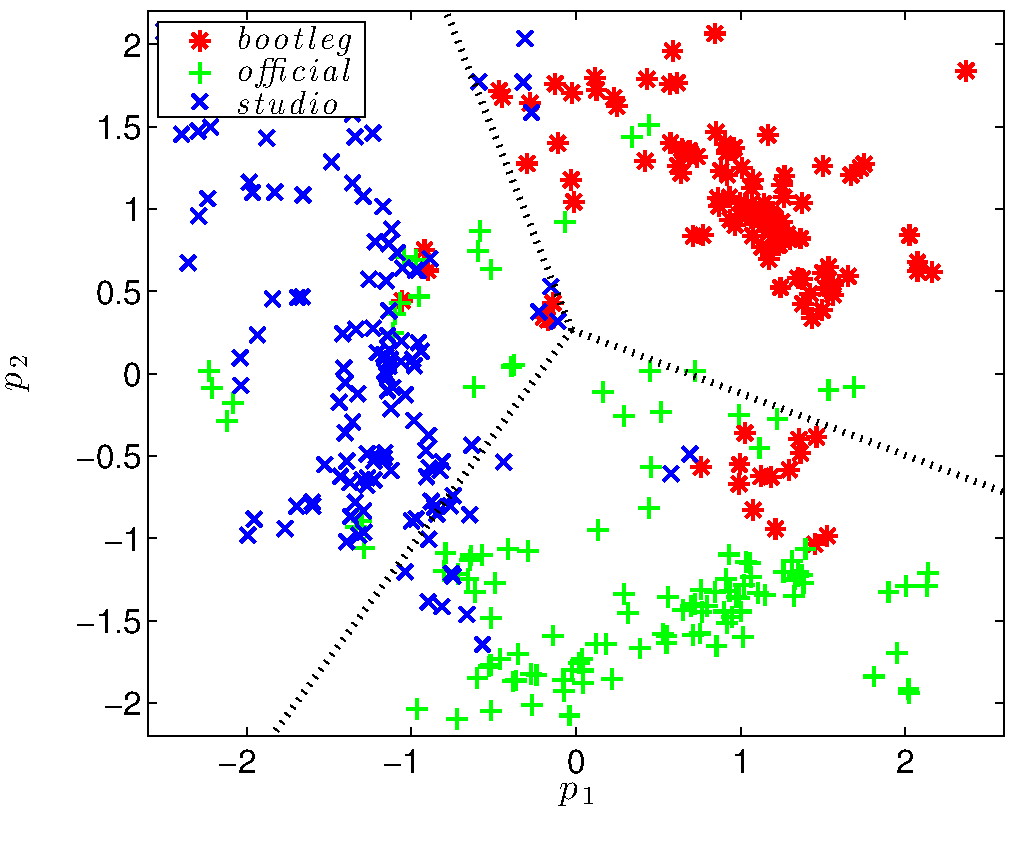
\includegraphics[width=.68\textwidth]{img/Bootleg/clusterDBN}\label{fig:Bootleg:clusterDBN}} \hfil
%\vspace{2em}
\centering
\subfloat[Hand-Crafted Features]{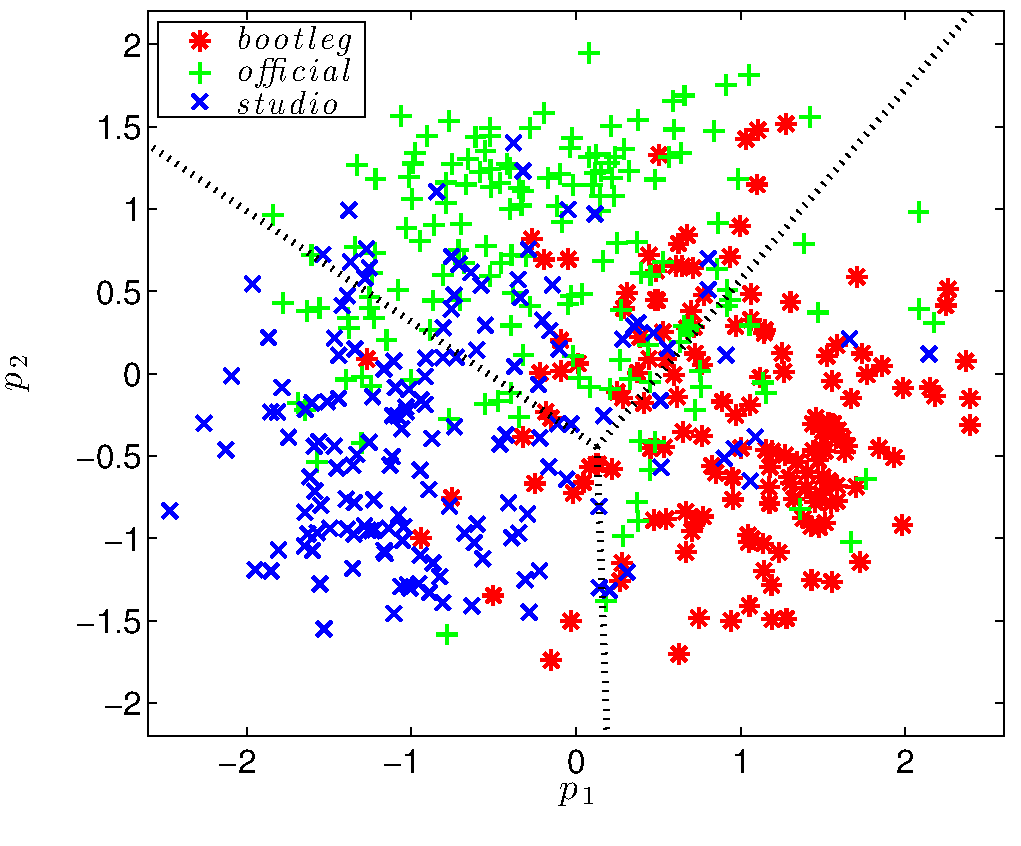
\includegraphics[width=.68\textwidth]{img/Bootleg/clusterHC}\label{fig:Bootleg:clusterHC}} \hfil
\caption{Visualization of learned (a) and hand-crafted (b) features projected along two dimensions $p_1$ and $p_2$. Notice how learned features are better clustered according to song classes. The Voronoi diagram according to clusters centroids is also shown (best seen in colors).}
\label{fig:Bootleg:clusters}
\end{figure}

Figure \ref{fig:Bootleg:clusters} shows the different clustering ability of hand-crafted and learned features. More specifically, we compared  vectors $\mathbf{h}^\text{(hc)}$ with vectors $\mathbf{h}^\text{(all)}$ extracted from the same songs in $\mathcal{S}$. For visualization purpose, we projected the features in a 2D space (i.e., $\operatorname{span}\{p_1, p_2\}$) that maximizes class separability in both cases. It is clear that learned features (Figure \ref{fig:Bootleg:clusterDBN}) separate the three classes better than hand-crafted features (Figure \ref{fig:Bootleg:clusterHC}).


\subsection{Numerical results}\label{sec:Bootleg:results}
To evaluate the classification method, we used the following metrics. Let us define $y_i \in \{\B, \O, \S \}$ the real class of the $i$-th song, and $\hat{y}_i$ its detected class. We evaluate the performance of the classification task with respect to the True Positives Rate (TPR), False Positives Rate (FPR), False Negatives Rate (FNR) and True Negative Rate (TNR) for each class. Given a generic class $\texttt{C}$ and $N$ the number of songs in $\STEST$, the four rates are computed as:
\begin{itemize}
\item TPR is the fraction of songs correctly classified into \texttt{C}:
\begin{equation}
TPR_{\texttt{C}}=\frac{ |\{y_i = \hat{y}_i = \texttt{C} \}|}{N};
\end{equation}
\item FNR is the fraction of songs incorrectly excluded from $\texttt{C}$
\begin{equation}
FNR_{\texttt{C}}=\frac{ |\{y_i = \texttt{C} \land \hat{y}_i \neq \texttt{C} \}|}{N};
\end{equation}
\item TNR is the fraction of songs correctly not classified into $\texttt{C}$
\begin{equation}
TNR_{\texttt{C}}=\frac{ |\{y_i \neq \texttt{C} \land \hat{y}_i \neq \texttt{C} \}|}{N};
\end{equation}
\item FPR is the fraction of songs incorrectly classified into $\texttt{C}$
\begin{equation}
FPR_{\texttt{C}}=\frac{ |\{y_i \neq \texttt{C} \land \hat{y}_i = \texttt{C} \}|}{N}.
\end{equation}
\end{itemize}
It is worth remembering that:
\begin{equation}
TPR_{\texttt{C}}+FPR_{\texttt{C}}+TNR_{\texttt{C}}+FNR_{\texttt{C}}=1 \; \forall \; {\texttt{C}} \in \{\B, \O, \S \}.
\label{eq:Bootleg:sumTFPN}
\end{equation}
From the four rates, we are able to compute the Precision, Recall and F-measure as described in Chapter \ref{Chap:HLFs}. %The Precision and Recall metrics do not take into consideration the True Negative Rate, since in several scenarios even a random predictor achieves high results for this metrics. In the scenario of classification into few labels, however, the True Negative Rate is as sensible as the other three rates. For this reason, 

We consider an additional performance metrics called Accuracy ($A$), which is computed as the fraction of the correctly classified samples, i.e.:
\begin{equation}
A_{\texttt{C}}=\frac{TPR_{\texttt{C}}+FPR_{\texttt{C}}}{TPR_{\texttt{C}}+FPR_{\texttt{C}}+TNR_{\texttt{C}}+FNR_{\texttt{C}}},
\end{equation}
where $A_{\texttt{C}}=TPR_{\texttt{C}}+FPR_{\texttt{C}}$ due to Equation \ref{eq:Bootleg:sumTFPN}. We compute the final Accuracy, Precision, Recall and F-measure as the average of the metrics over the three classes.

\begin{figure}[t]
\centering
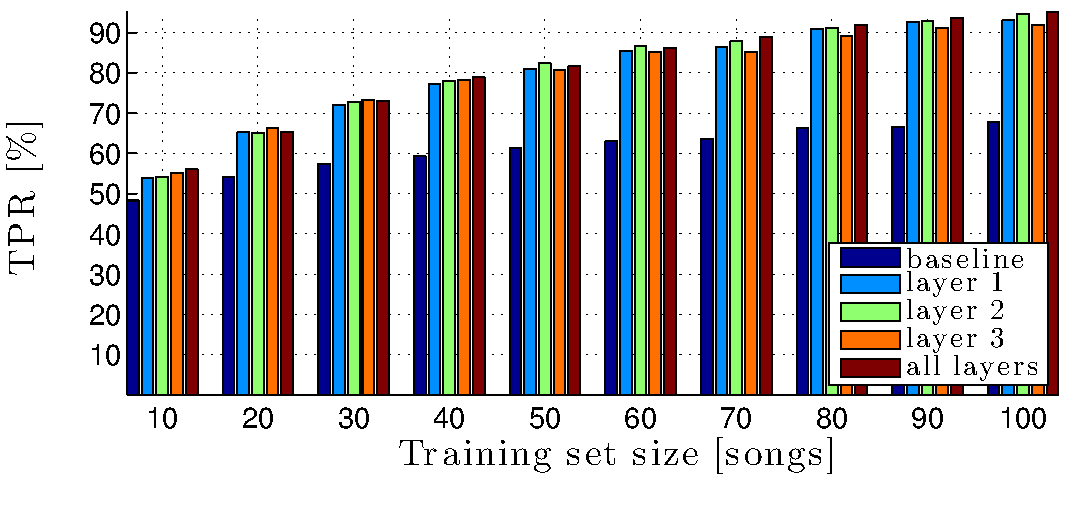
\includegraphics[width=.95\columnwidth]{img/Bootleg/succ_rate_bar}
\caption{TPR for different cardinality of the SVM training set size. Notice that, when using more than 80 songs, the trend remains quite constant.}
\label{fig:Bootleg:succ_rate}
\end{figure}

The performance of a system strongly depends on the size of the classifier's training set, i.e., it improves with the amount of data the classifier uses to learn a prediction model. Nevertheless Figure \ref{fig:Bootleg:succ_rate} shows the average TPR obtained with different learned feature vectors, as well as using the baseline method \cite{Bestagini2013b}, while changing the number of songs per class in $\Ssvm$. The sets of learned features clearly outperform the baseline method, especially with increasing training data. Moreover, we notice that after 80 songs per class in the training set, the TPR trend remains almost constant. For this reason, we decide to fix the cardinality of $\Ssvm$ to 80 songs per class for the following tests.



\begin{table}[t]
\caption{Confusion matrix comparison. Rows indicate the expected class, columns indicate the predicted class. For every class, the best and worst results in terms of TPR are highlighted in bold green and italics red, respectively. Results are expressed in percentage.}
\label{tab:Bootleg:conf_matrix}
\centering
%\large
%\small
\bgroup
\def\arraystretch{1.5}
\begin{tabular}{||c||c|c|c||c||}
\hline
\hline
$\quad \quad \quad$ & $\quad \hat{\B} \quad$ & $\quad \hat{\O} \quad$  & $\quad \hat{\S} \quad$  &  \\ 
\hline
\hline
 & {\color[HTML]{8E0000} \textit{72.81}} & {\color[HTML]{8E0000} \textit{18.25}} & {\color[HTML]{8E0000} \textit{8.94}}  & \textit{baseline}\cite{Bestagini2013b}   \\
  & {\color[HTML]{326B00} \textbf{96.70}} & {\color[HTML]{326B00} \textbf{1.10}}  & {\color[HTML]{326B00} \textbf{2.20}}  & \textit{layer 1}    \\
 $\B$ & 94.80  & 3.39 & 1.81 & \textit{layer 2}  \\
      & 94.60  & 3.30 & 2.10 & \textit{layer 3}  \\
      & 94.10  & 4.10 & 1.80 & \textit{all layers} \\
\hline 
& {\color[HTML]{8E0000} \textit{18.19}} & {\color[HTML]{8E0000} \textit{61.19}} & {\color[HTML]{8E0000} \textit{20.62}} & \textit{baseline}\cite{Bestagini2013b}   \\
& 3.20 & 85.00 & 11.80 & \textit{layer 1} \\
$\O$ & {\color[HTML]{326B00} \textbf{3.10}}  & {\color[HTML]{326B00} \textbf{87.60}} & {\color[HTML]{326B00} \textbf{9.30}}  & \textit{layer 2}    \\
& 3.90 & 83.90 & 12.20 & \textit{layer 3}  \\
& 2.80 & 87.50 & 9.70  & \textit{all layers} \\ 
\hline
  & {\color[HTML]{8E0000} \textit{12.00}} & {\color[HTML]{8E0000} \textit{22.88}} & {\color[HTML]{8E0000} \textit{65.12}} & \textit{baseline}\cite{Bestagini2013b}  \\
& 0.90 & 8.30 & 90.80 & \textit{layer 1} \\
$\S$ & 1.50 & 7.20 & 91.30 & \textit{layer 2}   \\
& 1.60 & 9.10 & 89.30 & \textit{layer 3}    \\
& {\color[HTML]{326B00} \textbf{0.50}}  & {\color[HTML]{326B00} \textbf{5.50}}  & {\color[HTML]{326B00} \textbf{94.00}} & \textit{all layers} \\ 
\hline

\end{tabular}
\egroup
\end{table}

Table \ref{tab:Bootleg:conf_matrix} reports the confusion matrix considering all the classes and all the proposed features sets, as well as the baseline method. We train the SVM over a random training set of songs, and perform the prediction over the resulting test set. We iterate the process of training and testing with a different random set of songs for each iteration, and we finally compose a confusion matrix with the averaged results over the iterations. The columns of the confusion matrix indicate the labels predicted by our system, which are compared with the expected labels, i.e., the labels in the ground truth, indicated by the rows. The main diagonal indicates the True Rates, while the other cells represent the False Rates. As an overall consideration, we notice that the SVM classifier is able to learn an effective model for all the features proposed, since the rate of the correctly detected labels is always higher than the sum of the false rates. 
We notice again that the approach based on learned features performs better than the approach based on hand-crafted ones. In particular, the baseline method performs worse than the proposed one on every class, whereas within the learned features, sometimes some specific layer of abstraction (i.e., $\mathbf{h}^{(1)}$, $\mathbf{h}^{(2)}$, and $\mathbf{h}^{(3)}$) obtains better results than the three layers stacked (i.e., $\mathbf{h}^{(all)}$). More specifically, it seems that the bootlegs are better detected with features learned from the first layer of the DBN, i.e., the least abstract ones, while official live recordings benefit from a slightly higher abstract representation. It is also worth noting that classification results do not depend on the length of feature vectors, since $|\mathbf{h}^{(1)}| < |\mathbf{h}^{(hc)}| < |\mathbf{h}^{(all)}|$.


\begin{table}[t!]
\vspace{5pt}
\caption{Evaluation comparison of the metrics True Positive Rate (TPR), Accuracy (A), Precision (P), Recall (R), F-measure (F). For every metric, the best and worst results are highlighted in bold green and italics red, respectively. Results are expressed in percentage.}
\label{tab:Bootleg:metrics}
\centering
%\large
\bgroup
\def\arraystretch{1.5}
\begin{tabular}{||c|c|c|c|c|c||}
\hline
\hline
\textbf{Model} & \textbf{TPR} & \textbf{A} & \textbf{P} & \textbf{R} & \textbf{F} \\ 
\hline
\hline
\textit{baseline} \cite{Bestagini2013b}   & {\color[HTML]{8E0000} \textit{66.38}} & {\color[HTML]{8E0000} \textit{77.58}} & {\color[HTML]{8E0000} \textit{66.43}} & {\color[HTML]{8E0000} \textit{66.38}} & {\color[HTML]{8E0000} \textit{66.38}} \\
\hline
\textit{layer 1}    & 90.83                                 & 93.89                                 & 90.87                                 & 90.83                                 & 90.81                                 \\
\textit{layer 2}    & 91.23                                 & 94.16                                 & 91.25                                 & 91.23                                 & 91.23                                 \\
\textit{layer 3}    & 89.27                                 & 92.84                                 & 89.28                                 & 89.27                                 & 89.25                                 \\
\textit{all layers} & {\color[HTML]{326B00} \textbf{91.87}} & {\color[HTML]{326B00} \textbf{94.58}} & {\color[HTML]{326B00} \textbf{91.94}} & {\color[HTML]{326B00} \textbf{91.87}} & {\color[HTML]{326B00} \textbf{91.87}} \\ 
\hline
\hline
\end{tabular}
\egroup
\end{table}

Finally, Table \ref{tab:Bootleg:metrics} shows all the defined metrics averaged on all the classes for every feature set. The metric results show that the classification based on learned features clearly outperform the system based on hand-crafted features. We notice that the middle layer (i.e., $\mathbf{h}^{(2)}$) exhibits slightly better performances than the other layers.
This may be due to the fact that footprints introduced by the bootleg or studio production are related to audio signal characteristics, rather than on high-level music abstraction, hence lower layers of the DBN are more effective in capturing them. Having stated the above, according to the proposed metrics, the use of $\mathbf{h}^\text{(all)}$ as feature vector is the best choice. In particular, it achieves performance above 90\%, and the accuracy is above 94\%. This means that the approach guarantees a almost perfect detection of bootleg recordings, also given the $TPR_{\B}=96.7 \%$ shown in Table \ref{tab:Bootleg:conf_matrix}.

\section{Final considerations}\label{sec:Bootleg:conclusion}
In this Chapter we explored the problem of the bootleg detection in order to build a system that is able to automatically recognize whether a song is an unauthorized live recording. 

The semantic domain is rather easy to formalize, since it is related to the process of recording of the songs, therefore it involves objective aspects and it does not require the modeling of the human perception. In fact, most of non-professional users might not be able to perceive whether a certain music track is a bootleg. On the other side, the signal domain is uncertain and not formalized, since it is hard to analyze which acoustic properties are affected in the generation of bootlegs and which features capture such properties. Finally, due to the uncertainty of the signal domain, it is also hard to design the linking function as a rule-based algorithm for this scenario.

As in Chapter \ref{Chap:MSA}, we addressed the issues raised by the formalization of the signal domain by learning a set of unsupervised features by means of a deep architecture. We have modeled the linking function as a machine learning technique as well, in order to learn the relationship between the signal domain and its semantic interpretation. 

Results on a dataset of nearly 500 songs confirmed that learned features better capture salient information about songs, thus making the approach more accurate than those based on hand-crafted features proposed in \cite{Bestagini2013b}. The obtained results are extremely high and nearly perfect. We believe that a deeper architecture or a supervised learning technique can walk the last mile for the problem. Nonetheless, the supervised approach is demanding of dedicated resources such as GPUs which were not available during this preliminary investigation.